
\begin{frame}{Bug}

  \begin{itemize}
   \item un \textbf{bug} (o \textbf{baco}) indica un errore o un comportamento inaspettato
   in un programma software;
   \item l'operazione di individuazione e correzione degli errori in un programma si chiama
   \textbf{debug}/\textbf{debugging};
   \item uno degli strumenti per facilitare l'operazione di debugging è il \textbf{debugging}
  \end{itemize}

\end{frame}

\pgfdeclareimage[width=0.25\paperwidth]{ada}{img/lovelace.jpg}
\begin{frame}{Bug (intermezzo storico) (I)}

  Piccola nota storica:
    \begin{columns}[T]
      \begin{column}{8cm}
	\begin{itemize}
	  \item in inglese \textbf{bug} significa \emph{insetto};
	  \item A livello teorico l'idea che un programma potesse contenere errori \`e stata avanzata
	  per la prima volta nel 1843 da \textbf{Ada Lovelace} nelle sue note sulla \textbf{macchina analitica} di \textbf{Babbage};
	  \item pare che l'espressione ``bug'' fosse in uso per indicare malfunzionamenti meccanici sin dal fine del 1800
	  (Thomas Edison, 1878)
	\end{itemize}

    \end{column}

    \begin{column}[T]{4cm}
	\begin{center}
	 \pgfuseimage{ada}
	\end{center}
    \end{column}
  \end{columns}


\end{frame}

\pgfdeclareimage[width=0.25\paperwidth]{bug}{img/bug.jpg}
\begin{frame}{Bug (intermezzo storico) (II)}

    \begin{columns}[T]
      \begin{column}{8cm}
	\begin{itemize}
    	  \item il primo bug informatico documentato della storia era un vero insetto (una falena),
	  che si era infilato in un rel\`e causando il malfunzionamento di un programma in un computer
	  all'università di Harvard, l'Harvard Mark II, il 9 settembre 1947. 
	  \item in seguito a quell'episodio il termine bug per indicare un problema informatico è diventato
	  comune grazie a \textbf{Grace Hopper} che era in capo al progetto Mark II.
	  (anche l'inventrice del primo compilatore).
	\end{itemize}
    \end{column}

    \begin{column}[T]{4cm}
	\begin{center}
	 \pgfuseimage{bug}
	\end{center}
    \end{column}
  \end{columns}

\end{frame}

\begin{frame}{Debugging (I)}

  \begin{itemize}
    \item durante il debugging un programma viene eseguito in modo interattivo per potere osservare
    l'esedcuzione del codice e il valore delle variabili passo dopo passo;
    \item si possono definire dei ``punti di controllo'', detti \textbf{breakpoints} e \textbf{watchpoints};
    \begin{itemize}
     \item nei \textbf{breakpoints} l'esecuzione di un programma viene interrotta per poterlo ispezionare;
     \item nei \textbf{watchpoints} l'esecuzione di un programma viene interrotta solo se una variabile
     viene letta o modificata;
    \end{itemize}

  \end{itemize}

\end{frame}

\pgfdeclareimage[width=0.5\paperwidth]{debug_breakpoint}{img/debug/debug_breakpoint.png}
\begin{frame}{Debugging (I)}

  \begin{itemize}
   \item Eclipse permette di lanciare un programma in \textbf{debug mode} e di usare una \textbf{debug perspective}
   allo scopo di eseguire il debugging;
   \item è possibile inserire un breakpoint cliccando all'inizio della riga con il tasto destro e selezionando
   \textbf{Toggle Breakpoint};
  \end{itemize}
  
  \begin{center}
   \pgfuseimage{debug_breakpoint}
  \end{center}

  \begin{itemize}
   \item Per lanciare il programma premere con il tasto destro sul nome del file e selezionare
   \textbf{Debug As $>$ Java Application};
  \end{itemize}

\end{frame}

% \pgfdeclareimage[width=0.25\paperwidth]{debug01}{img/debug/debug01.png}
{
  \setbeamercolor{background canvas}{bg=}
  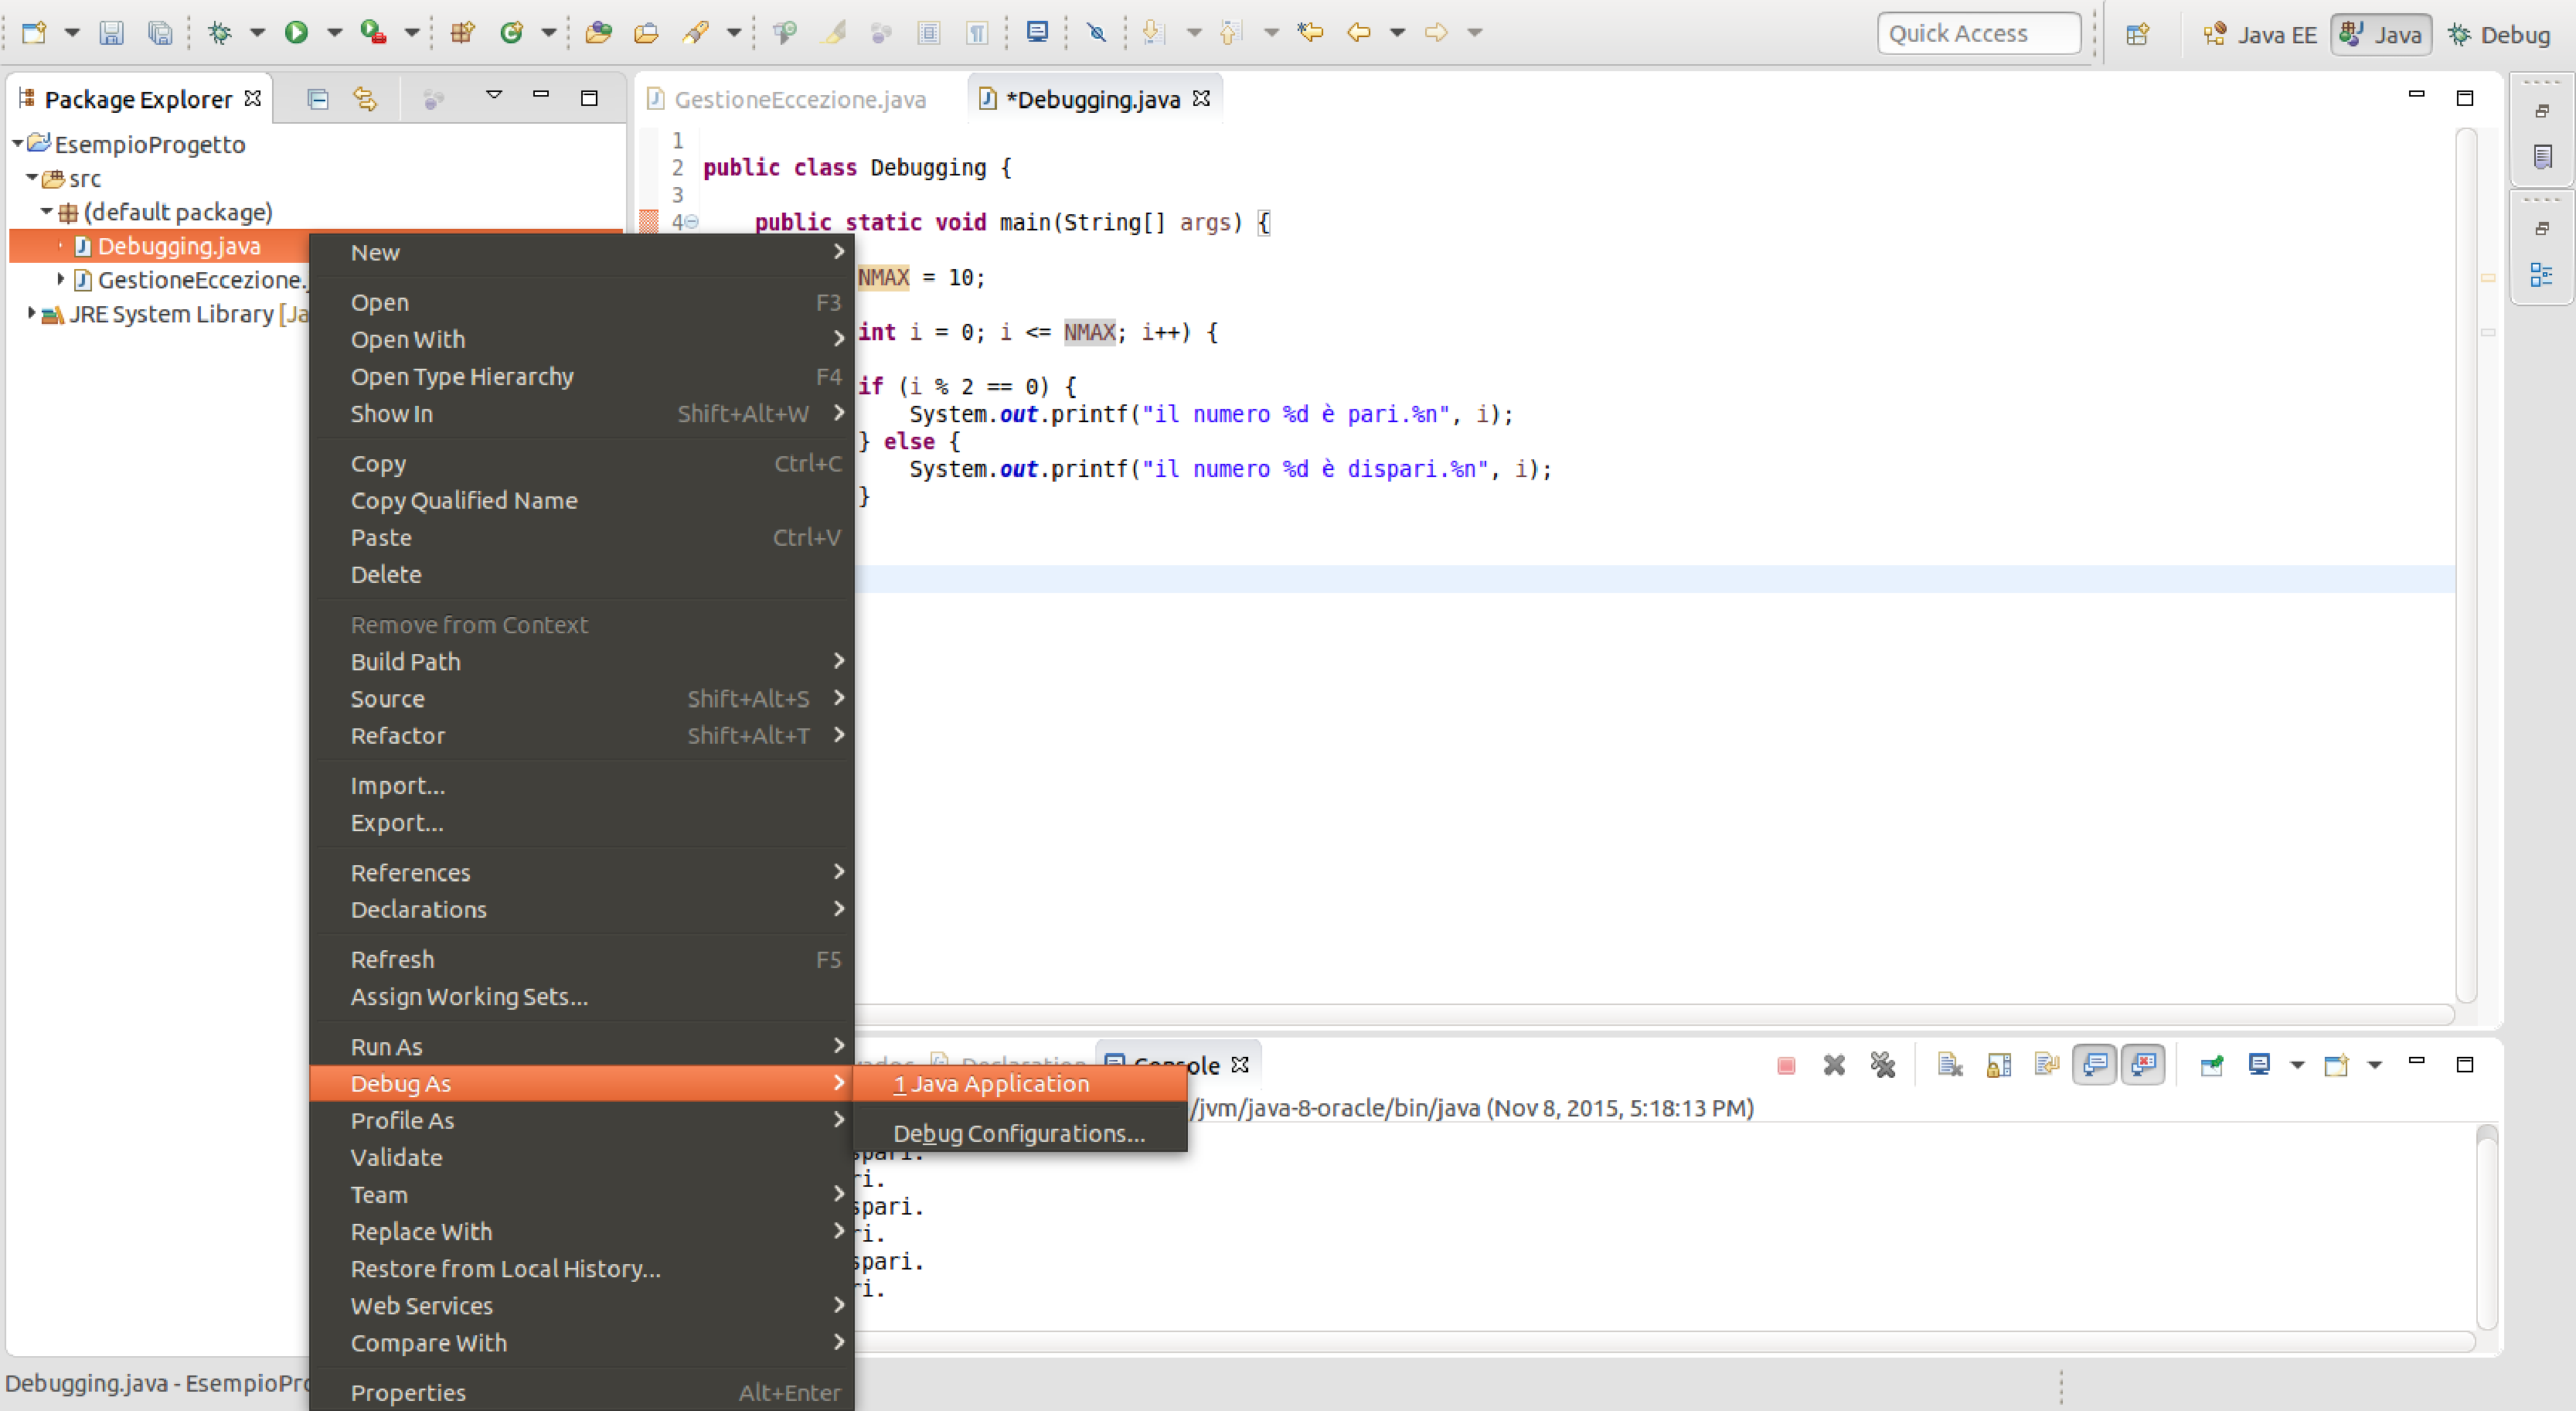
\includepdf[pages={1}]{img/debug/debug01.pdf}
}

\pgfdeclareimage[width=0.5\paperwidth]{debug_perspective}{img/debug/debug_perspective.png}
\begin{frame}{Debugging (II)}

  Confermare l'apertura della \emph{debug perspective}:
  \begin{center}
   \pgfuseimage{debug_perspective}
  \end{center}

\end{frame}

% \pgfdeclareimage[width=0.25\paperwidth]{debug01}{img/debug/debug01.png}
{
  \setbeamercolor{background canvas}{bg=}
  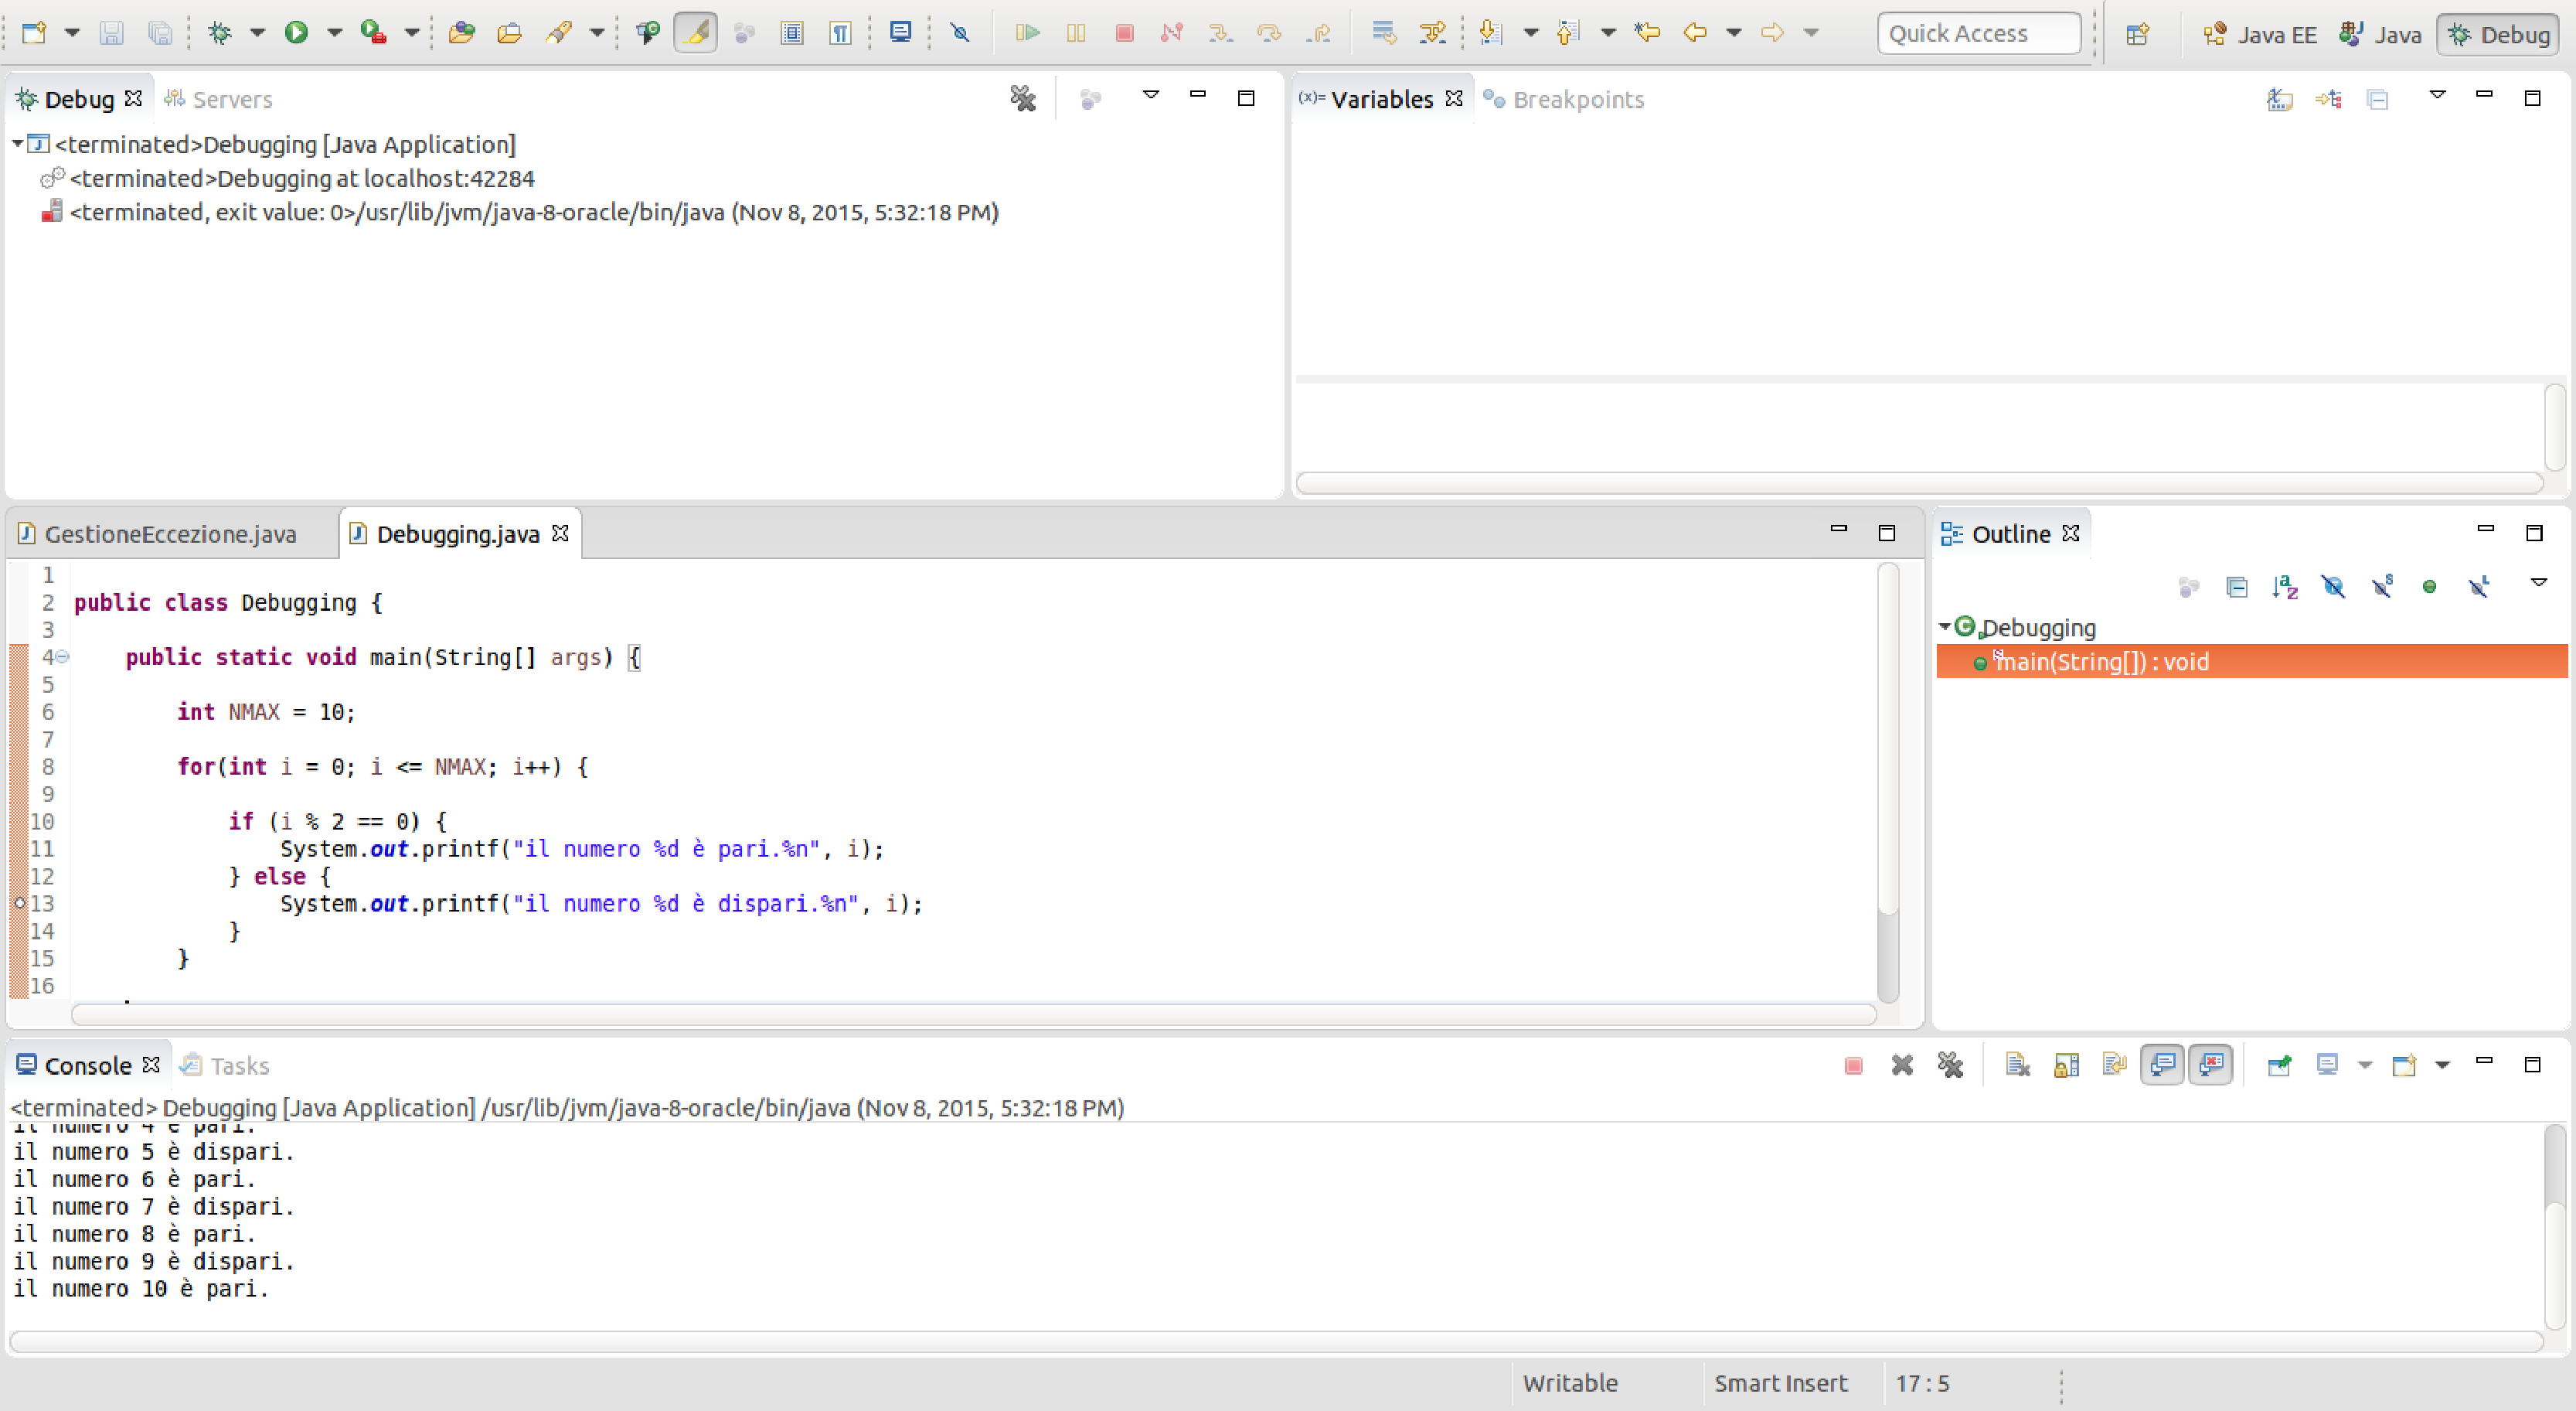
\includepdf[pages={1}]{img/debug/debug02.pdf}
}


\begin{frame}{Debugging (II)}

  Il debugger pu\`o essere comandato attraverso le icone nella barra o i tasti funzione:
  \begin{itemize}
    \item \textbf{F5} esegue la linea selezionata e va alla riga successiva. Se la linea selezionata \`e una chiamata a funzione allora il debugger entra nella funzione indicata;
    \item \textbf{F6} ``step over'': esegue un metodo senza entrare esplicitamente in esso con il debugger;
    \item \textbf{F7} ``step out'': ritorna alla funzione che ha chiamato il metodo corrent, ovvero termina l'esecuzione del metodo corrente e ritorna al chiamante;
    \item \textbf{F8} riprende l'esecuzione del programma fino a che non viene incontrato un nuovo breakpoint;
  \end{itemize}

\end{frame}

\begin{frame}{Debugging (III)}

  Dal pannello \textbf{variabili} è possibile:
  \begin{itemize}
    \item ispezionare il valore della variabile;
    \item (click destro) impostare un nuovo valore per la variabile;
  \end{itemize}

\end{frame}
